How transcription and further RNA processing can complexity the transcriptome even of the reduced organism

FLNC reads clustered to isoforms: 2.6M by 10 bps to 205k clustered; Use 10 for visual of 50 for operon backbone;  distribution of sharpness 5' and 3' ends

Find the longest RNA isoform for representative of operons; then merge and rescue to get total 480 operons

Statistics on operon size: operon can cover anti-sense genes; longest is rPtn operon; operon length distribution;

Promoter and terminator signatures: -10 box significant; -35 box not; terminator predicted as hairpins + polyU

\textit{Protein complexes in operons}

tRNAs in operons

Put one operon here: DCW operon?

% 5' and 3' UTRs

% Evaluate biological significance of gene co-expression: 

% \begin{itemize}
%     \item Glycolytic enzymes
%     \item rPtn operon
%     \item DNA replisome scattered (Angad commented)
% \end{itemize}

\begin{figure}[H]
    \centering
    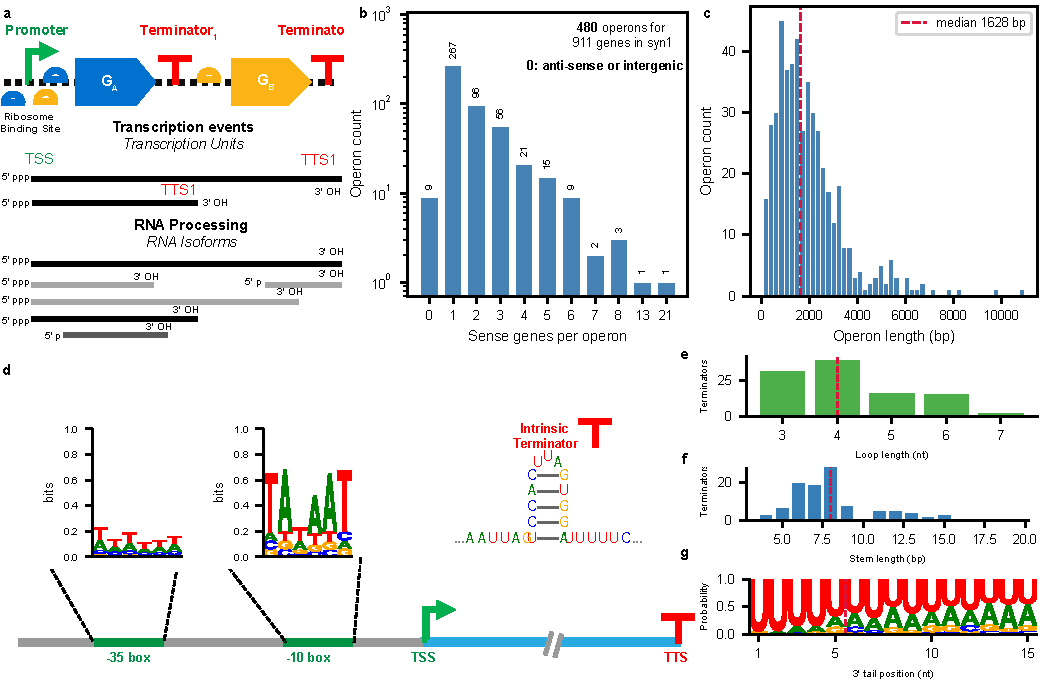
\includegraphics[width=1\linewidth]{figures/operon.pdf}
    \caption{Caption}
    \label{fig:placeholder}
\end{figure}

\textbf{Extended Figure:}

operon length distribution  

-35 region of TSS: not characteristic

tRNA in operons

\textbf{SI: Excel File Co-expression}

Sheet 1 operon candidate;

Sheet 2 protein complexes: operon, expression level; protein abundance

Sheet 3 tRNAs
